\section{Experiments And Evaluation}
\label{sec:exper}
In order to evaluate the proposed method for indoor scene segmentation, we conduct experiments on a publicly available benchmark dataset (NYUD-v2) and show the superiority of our method.
%, which contains 273 video sequences of RGBD data.  

\noindent\textbf{Dataset.}  
The NYUD-v2 dataset is a challenging dataset containing in total 464 diverse indoor scenes and the corresponding video sequences. 
%
For the task of semantic segmentation, only 1449 images are manually annotated, among which 795 images are used for training and the remaining 654 images for testing.
%
In our experiment, we map the semantic labels into 40 categories, similar as \cite{Gupta2014}.
%
From the 795 manually labeled images for training, we propagated these GT labels to 14344 unlabeled frames by setting the propagation range $K$ to 10, and filtered out 5897 frames by homography matrices, and filtered out 821 frames by manual check. 
We finally obtained 7626 frames with pseudo ground truth. 
%
Comparing with dense image annotation, filtering PGT for 273 videos merely took about 8 hours for a graduate student.
%
Although the generated pseudo labels still have a certain amount of noises, the diversity of training set is greatly enriched. 

The training images, including both manually labeled images and propagated images, are augmented by random horizontal flips with a possibility of 0.5, scaling with a randomly selected ratio in $\left\{0.7,0.8,0.9,1.0,1.1,1.2,1.3\right\}$ and random cropping. 
%
All our experiments are conducted on a single Nvidia Titan X Pascal GPU, using the Caffe framework.

\begin{figure}[!th]
	\centering
	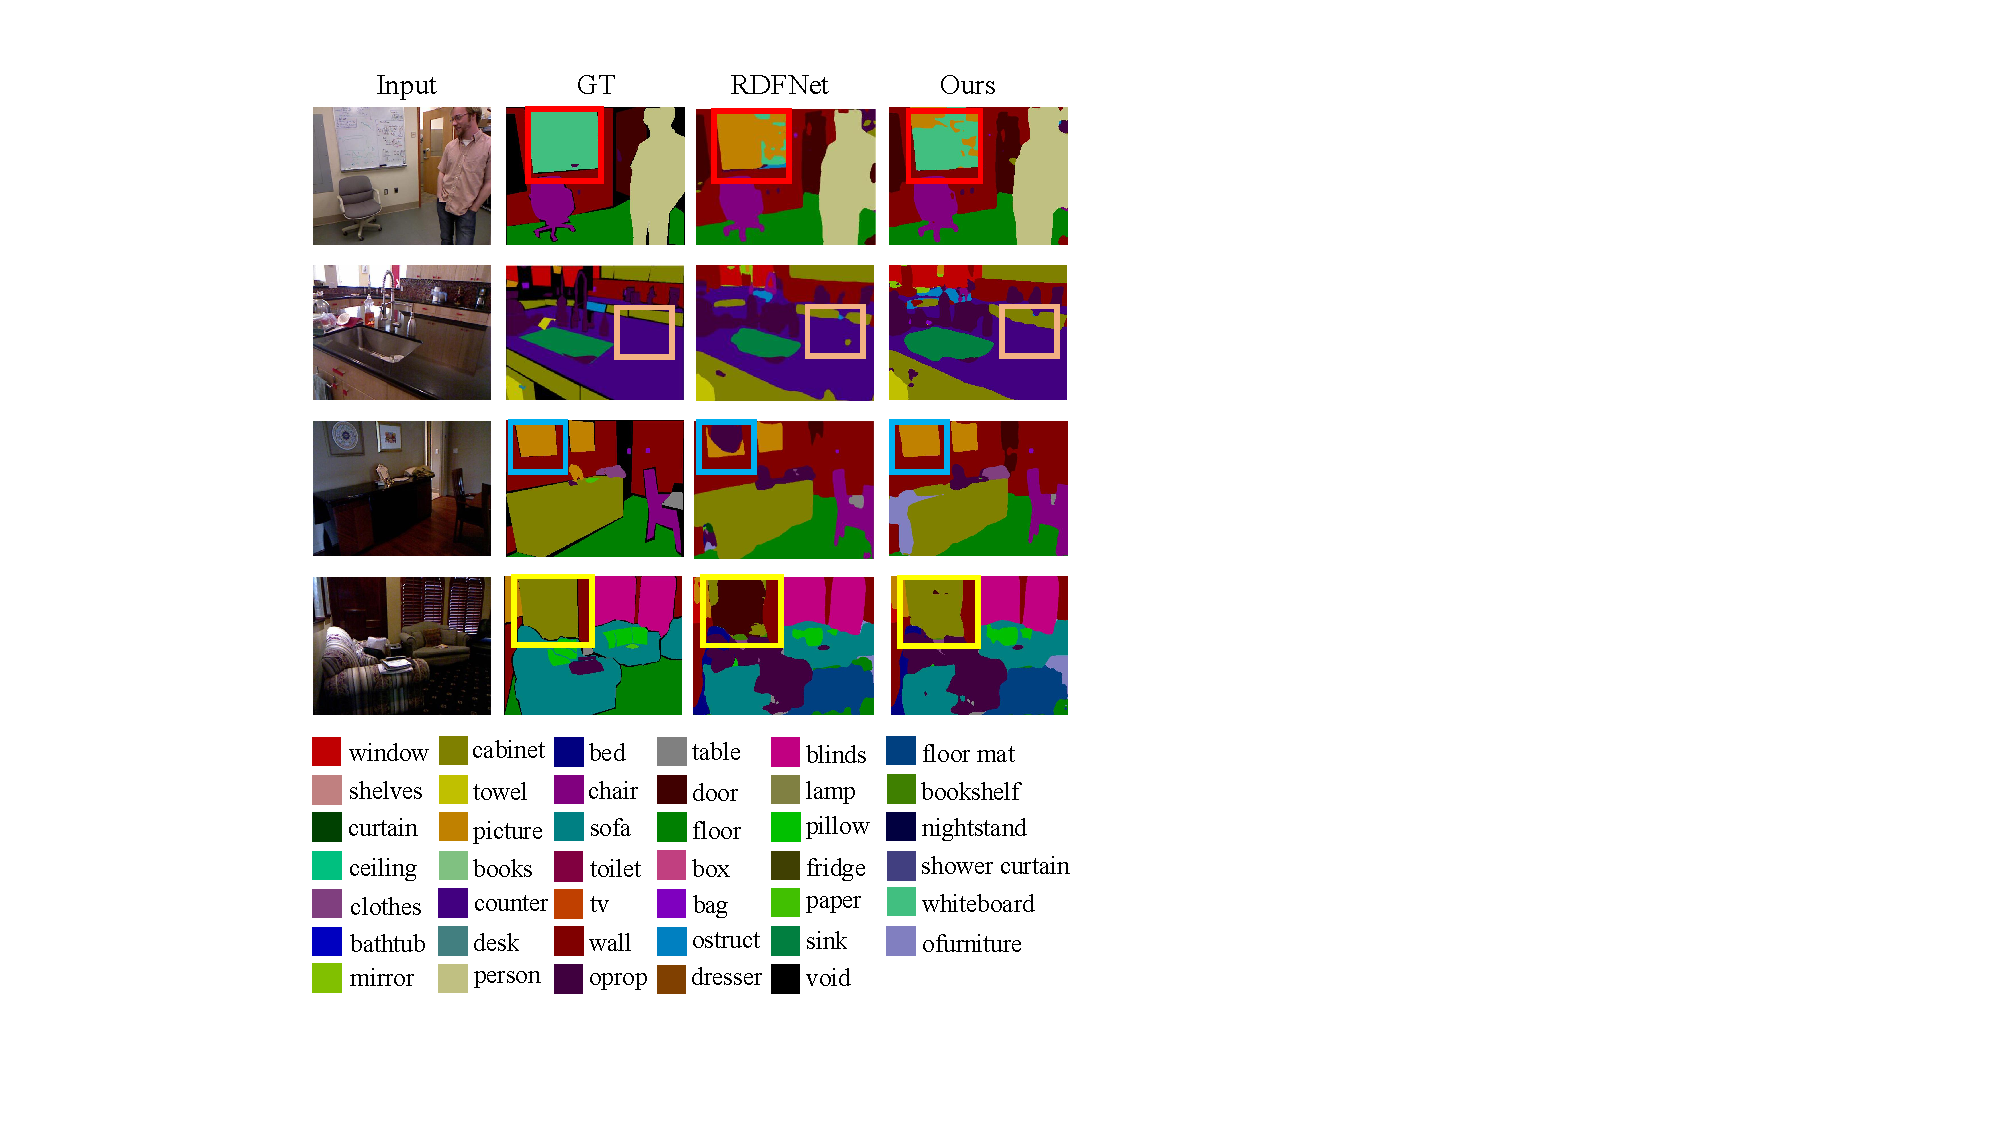
\includegraphics[width=\columnwidth]{figure/Result.pdf}
	\caption{Qualitative results on the NYUD-v2 dataset. In each row, we show the input image, the ground truth of semantic segmentation, the result of RDFNet, and the result of our method, from left to right, respectively. Our method predicts more accurate segmentation results, especially at the highlighted regions.}
	\label{fig:VisResult}
	\vspace*{-0.3cm}
\end{figure}


\noindent\textbf{Evaluation Metrics.}  
Following previous work
\cite{Eigen2015,Gupta2014,Kendall2015,Lin2016,Lin2017,Li2016,Cheng2017,Park2017,Xu2018,Zhang2018,Jiao2018}, we use three quantitative metrics to evaluate our semantic segmentation results, including pixel accuracy, mean accuracy and mean Intersection over Union (mIoU). 
%%
Denote $m_{kj}$ as the number of pixels of class ${k}$ classified as class ${j}$.
%Assuming 
The number of categories is $c$, and $M_{k} = \sum_{j}m_{kj}$ is the total number of pixels belonging to class $k$. 
%
And $N = \sum_{k}M_{k}$ denotes the number of all pixels in the test set.
%
The three metrics are defined as follows:
\begin{equation}\label{eq:metric}
\begin{array}{rl}
\text{pixel accuray}: &  \frac{1}{N}\sum_{k}m_{kk}, \\
\text{mean accuracy}: &\frac{1}{c}\sum_{k}\frac{m_{kk}}{M_{k}}, \\
\text{mean IoU}: &\frac{1}{c}\sum_{k}\frac{m_{kk}}{ M_{k}+\sum_{j}m_{jk}-m_{kk}}.
\end{array}
\end{equation}

\begin{table}[tb]
%	\vspace{-0.4cm}
	\centering
	\caption{Comparison of different methods. The three columns represent three different types of methods: semantic segmentation of a single image, semantic segmentation of RGBD images and multi-task learning methods.}
	\begin{tabular*}{8.2cm}{llccc}
		\hline
		Method & Data & Pixel & Mean  & Mean\\
		       &     & accuracy & accuracy  & IoU \\
		\hline 
		B-SegNet \cite{Kendall2015} & RGB &68.0 & 45.8 & 32.4 \\
		Context \cite{Lin2016} & RGB & 70.0 & 53.6 & 40.6 \\
		RefineNet \cite{Lin2017} & RGB & 73.6 & 58.9 & 46.5\\
		\hline
		Gupta et al. \cite{Gupta2014} & RGBD & -- & 35.1 &--\\
		Eigen et al. \cite{Eigen2015} & RGBD & 65.6 & 45.1 & 34.1\\
		FCN \cite{Long2015} & RGBD & 65.4 & 46.1 & 34.0 \\
		LSTM-CF \cite{Li2016} & RGBD & --& 49.4 & -- \\
		Cheng et al.\cite{Cheng2017} & RGBD & 71.9 & 60.7 & 45.9 \\
		RDFNet \cite{Park2017} & RGBD & \bf{76.0} & 62.8 & 50.1\\	
		%\hline
		Baseline &RGBD & 75.8 & 63.0 & 50.0\\
	%	Flow-PGT & RGBD & & &\\
		Ours (+$L_{C}$) & RGBD & 75.8 & 63.3 & 50.1\\	
		Ours (+$Pr$) & RGBD & 75.5 & 63.5 & 49.8\\
	%	Ours(+$Hm$) & RGBD & & &\\
		Ours (+$PGT$) & RGBD & 75.9 & 63.6 & 50.2\\
		Ours (+$L_{C}$+$PGT$)& RGBD & 75.8 & \bf{63.8} & \bf{50.2}\\
		\hline
		PAD-Net \cite{Xu2018} & RGB &75.2 & 62.3 & 50.2\\
		TRL \cite{Zhang2018} & RGB &76.2 & 56.3 & 46.4\\
		Jiao et al.\cite{Jiao2018} & RGB & \emph{81.1} & 62.2 & \emph{50.9}\\
		\hline		 		
	\end{tabular*}
	\label{Tab:Results}
\end{table}

We set the RDFNet~\cite{Park2017} as our baseline. 
However, due to hardware difference, using the official code, we get results (Baseline) that is slightly different from that reported in their paper (RDFNet), as shown in Table~\ref{Tab:Results}. 
We compare different variants of our approach to demonstrate the effectiveness of each component, and the results are reported in Table~\ref{Tab:Results}. 

\para{Analysis of Pseudo labels.} 
Though the pseudo labels still contain a certain amount of noises, most of them are reliable, especially inside on object region. 
%
While training the RDFNet with extra images of pseudo labels, the performance (+PGT for short) greatly increases, especially at mean accuracy ($63.6\%$), compared with the baseline.
%
In addition, we investigate the effect of quality of PGT on network performance.
%
Simply limiting the range of annotation propagation, the performance of baseline method begins to decline, largely due to the poor quality of PGT.
%
But on the other hand, with the increase of the number of coarsely annotated training samples, the performance (+Pr for short) of obtained model for each category (Mean accuracy) is improved.

\para{Analysis of Temporal Consistency.} While training RDFNet with the 795 manually labeled images, and our temporal consistency constraint (+$L_C$ for short), the mean accuracy increases to $63.3\%$ from $63.0\%$, and mIoU increases to $50.1\%$ from $50.0\%$. 
%
The results show that training the network with self-supervised loss function could effectively improve the performance of fully supervised baseline method.

\begin{table*}[h]  
	\caption{Class-wise IoU on NYUD-v2}  
	\centering
	\normalsize
	%\setlength{\tabcolsep}{1mm}{
	\begin{tabular*}{16.3cm}{l|cccccccccc}  
		\hline		
		&wall &floor &cabinet &bed &chair&sofa& table& door & window& bkshelf\\   
		\hline  
		RDF-152 & 79.7 & 87.0 & \bf{60.9} & \bf{73.4}& \bf{64.6}& \bf{65.4}& \bf{50.7}& 39.9 & 49.6& 44.9\\
		Ours & \bf{80.8} & \bf{87.9} & 60.1 & 72.1& 64.1& 64.6 & 49.2 & \bf{41.6}
		& \bf{49.8}& \bf{45.3}\\
		\hline  
		\hline 
		 & counter & blind & desk& shelf&curtain& dresser& pillow& mirror& mat&cloths\\
		\hline 
		RDF-152& \bf{67.1}& \bf{63.9}& \bf{28.6}& 14.2 & 59.7&\bf{49.0} & 49.9 & 54.3& 39.4 & 26.9 \\
		Ours  & 66.6 & 61.9 & 25.1& \bf{14.4}& \bf{59.9} & 46.2 & \bf{50.1} & \bf{55.9}& \bf{41.5}&\bf{27.4}\\
		\hline 
		\hline 
		& books& refridge& tv&paper& tower& shower& box& board&person& stand\\ 
		\hline 
		RDF-152 & \bf{35.0} & 58.9& \bf{63.8} & \bf{34.1} & 41.6 & \bf{38.5} & 11.6& 54.0& 80.0 & \bf{45.3}\\ 
		Ours& 34.7 & \bf{61.4} & 61.9& 32.9 & \bf{41.7} & 37.0 & \bf{11.9}& \bf{56.8}& \bf{82.4} & 44.5\\
		\hline 
		\hline 
		& sink& lamp&bathtub& bag& othstr& othfurn& othprop& picture& ceiling& toilet\\
		\hline
		RDF-152   & 62.1& 47.1& 57.3 & 19.1 & 30.0 & 20.6& \bf{39.0}& 61.2& \bf{69.1}& 65.7\\
		Ours & \bf{65.3}& \bf{47.2}& \bf{58.5} & \bf{19.9} & \bf{32.3} & \bf{20.8}& 38.1& \bf{61.7}& 68.9 & \bf{66.5}\\
		\hline 
		\hline
	\end{tabular*}
	\label{Tab:Results_classes}
\end{table*}

Combining both the pseudo ground truth and temporal consistency, our approach outperforms existing semantic segmentation networks, especially at mean accuracy and mIoU metrics. 
%
We also compare our method with three multi-task learning techniques and our method achieves comparable performance.
%
Though Jiao \emph{et al.} achieve the best performance on pixel accuracy and mIoU, they require additional dense ground-truth for depth estimation and much heavier computational cost.
%
Fig.~\ref{fig:VisResult} shows a group of segmentation results. It can be seen that our method performs well on objects such as pictures, whiteboards and so on. 
%
And compared with baseline method, there is less over-segmentation in our approach, such as picture on the walls (Fig.~\ref{fig:VisResult}, line 3) and cabinet in the corner (Fig.~\ref{fig:VisResult}, line 4).
%
Class-wise IoU of our results compared with RDFNet\cite{Park2017} are shown in Table~\ref{Tab:Results_classes}.
%
The experimental results in Table~\ref{Tab:Results_classes} show that our method effectively improves segmentation accuracy on most categories (24/40) by using label propagating and self-supervised loss function.
%
It's not only in categories with large planes such as wall, floor and door, but also in classes with small size such as bag and box. 
%
Although our method improves the performance of small objects, the mIoU of box and bag are still under $30\%$. 
%
The main reasons are that the size of these two kinds of objects is too small and the occurrence frequency of them is very low ($<25\%$).
%


\begin{comment}
\para{Analysis of Temporal Consistency.}  
To discover the effectiveness of our proposed training policy. 
%
We conduct our experiments on generated PGT data with temporal consistency loss.
%
The quantitative and qualitative results are shown in Table~\ref{Tab:Results} and
Fig.~\ref{fig:VisResult} respectively.
%
To prove that performance improvements are not just due to PGT, we did an ablation study by removing ${PGT}$.
%
The results are shown in Table~\ref{Tab:Results} and Fig.~\ref{fig:VisResult}.
%
Compared to baseline, the mean accuracy and IOU are all been promoted.
%
Using $L_{consistency}$ and $L_{PGT}$ simultaneously, the mean accuracy is improved by 0.8\%.
%
And mean IoU is improved by 0.2\%.
%
And our method achieves the comparable performance as multi-task learning method.
}
\end{comment}


\para{Discussion.} By involving temporal consistency, we also found that there are conflicts between manual labels of the same scene, as shown in Fig.~\ref{fig:mislabels}. 
%
Compared to other methods, our approach produces much more accurate and consistent results that shown in Fig.~\ref{fig:mislabels}(e).
%
And the feature extracted by our model is much more robust.
%
%The mean accuracy and mean IoU are under 30\%.
%
% the ground truth proposed by NYUD-v2 data set exits some annotation errors shown in Fig.~\ref{fig:mislabels}.


\begin{figure}[!htbp]
	\setlength{\abovecaptionskip}{-0.2cm}
	\setlength{\belowcaptionskip}{-10cm}
	\centering
	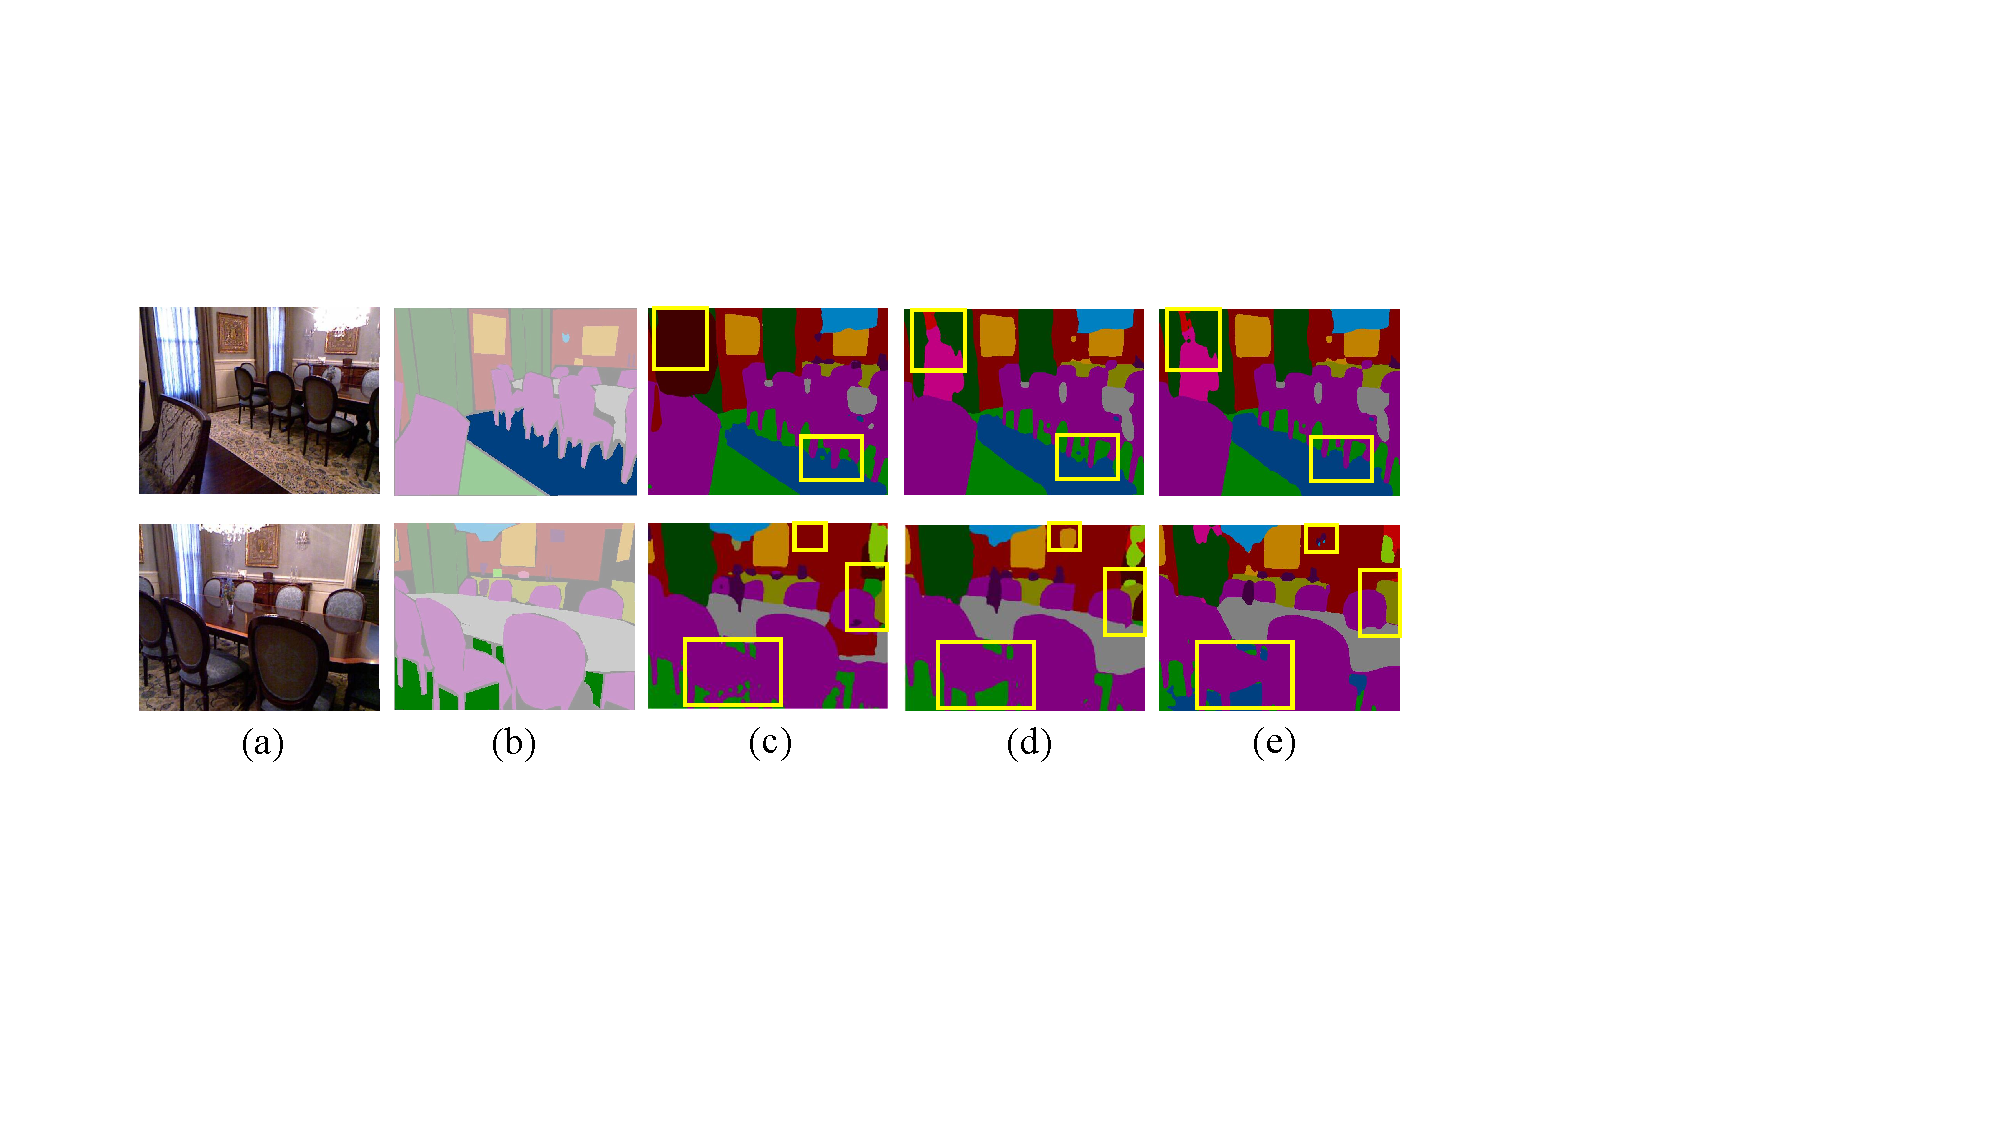
\includegraphics[scale=0.4]{figure/Mislabels.pdf}
	\caption{Mislabeled images. (a) Two frames of the same scene. (b) Their corresponding ground truth labels. Note the difference between the labels of the floor pixels. Blue as "floor mat" and green as "floor".  The mislabeled pixels are highlighted. (c)(d)(e) The prediction results of RefineNet, RDFNet and our method, respectively. The details are framed in yellow.}
	\label{fig:mislabels}
\end{figure}
%

\begin{comment}{
But our proposed method shows a more robust result compared to RefineNet \cite{Lin2017} and RDFNet \cite{Park2017}.
%
}
\end{comment}





